\section{Methodology}
\label{method}
In this section, we define the task and present our proposed Dual-Granularity Gaussian Contrastive Learning (DGGC) model, where the overview of DGGC is illustrated in Figure \ref{fig:over}. We first define the table union search task in Section \ref{sub_pre}. Then we describe the dual-granularity encoder, which explicits tables' and columns' semantic specificity distributions, including a mean embedding and a variance embedding (Section \ref{sub_sec_dul}). Additionally, we design the training loss of Gaussian contrastive learning model (Section \ref{sub_sec_gau}). In Section \ref{sub_sg}, we introduce a filter-shuffle sample generator to expand the positive samples to address the self-referential bias in contrastive learning. The overall training process is presented in Section \ref{sub_sec_over}. Finally, we provide the unionability score between columns and tables for the online search process (Section \ref{sub_sec_onl}).

\subsection{Task Definition}
\label{sub_pre}
\begin{figure*}[t]
    \centering
    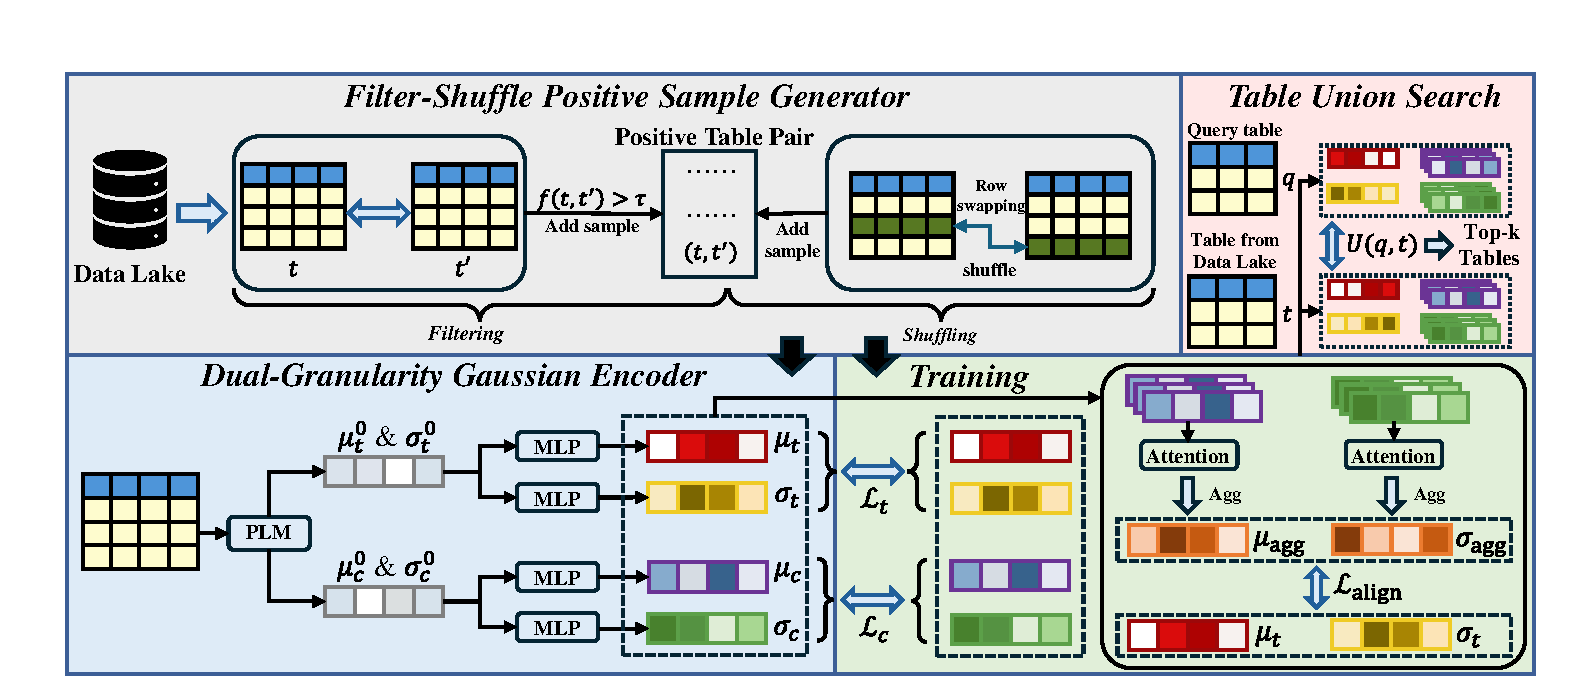
\includegraphics[width=\textwidth]{figure/overview.pdf}
   \caption{
\textbf{The framework of DGGC.} DGGC encodes tables and columns into mean and variance embeddings, uses a filter-shuffle mechanism to generate cross-table positives, and optimizes Gaussian-specific losses for online unionability ranking.
}
    \label{fig:over}
\end{figure*}
Following SANTOS~\cite{khatiwada2023santos}, we adopt a relationship-based semantic definition of unionability. A table is a set of columns $\{c_1,\dots,c_n\}$, each possibly from a distinct domain. Given a query table $q$ and candidate table $t$, $t$ is unionable with $q$ if columns in $q$ can be one-to-one matched to a subset of columns in $t$ while preserving semantic types and inter-column relationships. Accordingly, $U(q,t)$ denotes the semantic unionability degree of $t$ with respect to $q$.
Given a query table $q$ and a table corpus ${T}$, table union search aims to return a top-$k$ list of tables $\{t_1,\dots,t_k\}$ from ${T}$, such that $\forall t\in\{t_1,\dots,t_k\}$ and $\forall t'\in {T}\backslash \{t_1,\dots,t_k\}$, $U(q,t)\geq U(q,t')$.
\subsection{Dual-Granularity Gaussian Encoder}
\label{sub_sec_dul}
Although table union search is typically determined by column similarity, relying solely on column-level representations may ignore global table semantics that provide contextual constraints. To capture both local attribute semantics and global contextual information, we design a dual-granularity Gaussian encoder that models tables and columns simultaneously. To further model semantic specificity beyond deterministic embeddings, we represent each table or column embedding \(x\) as a diagonal Gaussian distribution:
\begin{equation}
\label{eq_gaussian_embedding}
    \mathcal{N}_x
    =
    \mathcal{N}
    \left(
    \mathbf{\mu}_x,
    \mathbf{\Sigma}_x
    \right),
    \qquad
    \mathbf{\Sigma}_x
    =
    \mathrm{diag}(\mathbf{\sigma}_x^2).
\end{equation}
where $\mu_x \in \mathbb{R}^d$ denotes the mean embedding
and $\Sigma_x = \mathrm{diag}(\sigma_x^2)$ is a diagonal covariance matrix. Unlike deterministic embeddings, Gaussian representations allow each table or column to occupy a semantic region in latent space.

We adopt diagonal covariance for scalability, reducing parameter complexity from \(O(d^2)\) to \(O(d)\) and enabling efficient closed-form distance computation.

\noindent\textbf{Initialization.} 
We initialize representations using RoBERTa~\cite{liu2019roberta}, a widely adopted pre-trained language model with strong contextual encoding capability. Pre-trained language models provide rich lexical and contextual priors, which are particularly important for modeling heterogeneous and noisy cell values in data lakes {\cite{yin2020tabert,deng2022turl}}. Each column \(c_i\) is serialized into a sentence \(s_i\) by concatenating its cell values. All column sentences are then organized and the whole table is encoded as $\text{PLM}(\text{[CLS]}\ s_1\ \text{[SEP]} \dots \text{[SEP]}\ s_n \ \text{[SEP]})$, 
where the [CLS] token represents the table-level embedding and each segment corresponds to a column. The PLM output provides initial mean and variance embeddings for both table- and column-level representations, i.e., $\mathbf{\mu}_{t}^0$, $\mathbf{\sigma}_t^0$. For column-level embeddings, the PLM outputs embeddings for each column segment, which are taken as the initial mean $\mathbf{\mu}_{c}^0$ and variance $\mathbf{\sigma}_c^0$ for each column $c$. It is important to note that our approach is applicable to other BERT variants as well. 

\noindent\textbf{Gaussian Layer.} 
After PLM initialization, we use a Gaussian Layer to refine the Gaussian parameters of tables and columns. To avoid ambiguity, we explicitly define four MLP projection functions:
\(\mathrm{MLP}_{t}^{\mu}\), $\mathrm{MLP}_{c}^{\mu}$, $\mathrm{MLP}_{t}^{\sigma}$ and $\mathrm{MLP}_{c}^{\sigma}$. 
The subscript \(t\) or \(c\) denotes the granularity of the input representation, namely table-level or column-level. The superscript \(\mu\) or \(\sigma\) denotes the Gaussian parameter branch, namely the mean branch or the variance branch. Parameters are not shared across granularities or branches to preserve their distinct semantic roles.

For the \(l\)-th Gaussian layer, the mean embeddings are updated as \({\mathbf{\mu}}_{t}^{l+1}=\mathrm{MLP}_{t}^{\mu}(\mathbf{\mu}_{t}^{l})\) and \({\mathbf{\mu}}_{c}^{l+1}=\mathrm{MLP}_{c}^{\mu}(\mathbf{\mu}_{c}^{l})\). Similarly, the variance embeddings are updated as \(\mathbf{\sigma}_{x}^{l+1}=\phi_{\sigma}(\mathrm{MLP}_{x}^{\sigma}(\mathbf{\sigma}_{x}^{l}))\), where \(x \in \{t, c\}\) and \(\phi_{\sigma}\) is a positive activation (e.g., softplus) ensuring valid covariance. In our implementation, \(\phi_{\sigma}\) is instantiated as a softplus function with a small constant \(\epsilon\), i.e., \(\phi_{\sigma}(x)=\mathrm{softplus}(x)+\epsilon\). This positivity constraint guarantees that the diagonal covariance matrix \(\mathbf{\Sigma}_x=\mathrm{diag}(\mathbf{\sigma}_x^2)\) is valid for each table or column Gaussian embedding. Consequently, each table or column is not represented as a single deterministic point, but as a Gaussian distribution with a semantic center \(\mathbf{\mu}_x\) and a specificity-aware covariance parameterized by \(\mathbf{\sigma}_x\).


\subsection{Contrastive Training}
\label{sub_sec_gau}
After obtaining Gaussian embeddings at both table and column granularities, we optimize DGGC with three objectives: table-level contrastive loss, column-level contrastive loss, and a table–column alignment loss. Given a query table \(q\), its unionable tables are treated as positive samples \(\{t_1^+, \dots, t_P^+\}\), while non-unionable tables form the negative set \(\{t_1^-, \dots, t_N^-\}\). The table-level contrastive loss is defined as:
\begin{equation}
\label{eq_cl}
    \mathcal{L}_t=-\log\frac{\sum_{p=1}^P\exp(\mathcal{G}(q,t_p^+))}{\sum_{p=1}^P\exp(\mathcal{G}(q,t_p^+))+\sum_{n=1}^N\exp(\mathcal{G}(q,t_p^-))}    
\end{equation}
For the score function between $q$ and its samples $t$, we adopt the Wasserstein-2 distance as our geometric loss function for Gaussian embedding learning \cite{muzellec2018generalizing}. To flexibly control the relative importance between semantic center alignment and specificity consistency, we introduce a scaling parameter $\lambda$ and define a generalized Wasserstein distance. Given the Gaussian embeddings $\mu_q$, $\sigma_q$ and $\mu_t$, $\sigma_t$ for $q$ and $t$ respectively, we adopt the squared 2-Wasserstein distance between the two Gaussian distributions and convert it into a compatibility score for contrastive learning:
\begin{equation}
\label{eq_gs}
    \mathcal{G}(q,t)=-
    \underbrace{{||\mu_q-\mu_t||_2^2}}_{\text{mean distance}}-\underbrace{\lambda\cdot||\sigma_q-\sigma_t||_2^2}_{\text{variance distance}} 
\end{equation}
where the first term aligns semantic centers and the second enforces consistency of semantic specificity. If the two tables should not be unioned, a penalty of semantic specificity is applied to account for discrepancies in semantic specificity {\cite{vilnis2014word}}. 
The hyperparameter \(\lambda\) controls the relative importance of mean similarity and variance alignment. The introduction of the parameter $\lambda$ serves to balance the importance of mean similarity and variance distance, enabling fine-tuning of the model's sensitivity to semantic discrepancies. The contrastive loss for columns, $\mathcal{L}_c$, is defined analogously to Eq. \eqref{eq_cl} and \eqref{eq_gs}.

To ensure consistency between global table semantics and local column semantics, we aggregate column embeddings within table \(t\). 
For each column \(c \in t\) with Gaussian embedding \((\mu_c, \sigma_c)\), we compute an aggregated table-level representation via attention, where \(\mu_{\text{agg}} = \text{Attn}_{\mu}(\{\mu_{c}\}_{c\in t})\) and \(\sigma_{\text{agg}} = \exp(\text{Attn}_{\sigma}(\{\log\sigma_{c}\}_{c\in t}))\). Here, $\text{Attn}_{\mu}$ and $\text{Attn}_{\sigma}$ are attention functions that compute weighted sums of input embeddings. Using the logarithmic form of variance embeddings stabilizes the variance values and ensures that they are positive, thereby facilitating effective aggregation during the attention computation. Given the Gaussian embedding $\mu_t$ and $\sigma_t$ of table $t$, we define the alignment loss as $\mathcal{L}_{\text{align}}=||\mu_t-\mu_\text{agg}||_2^2+\lambda||\sigma_t-\sigma_\text{agg}||_2^2$. The loss $\mathcal{L}_\text{align}$ reinforces the association of semantic specificity distribution between table and its columns. The total loss is defined as:
\begin{equation}
\label{eq_loss}
\mathcal{L}=\mathcal{L}_t+\alpha\mathcal{L}_c+\beta\mathcal{L}_\text{align}
\end{equation}
where $\alpha$ and $\beta$ are weights to balance different losses.

\iffalse
\subsection{Filter-Shuffle Positive Sample Generator}
\label{sub_sg}
A central difficulty in contrastive learning over heterogeneous tables is \emph{self-referential bias}, where only augmented views of the same table are treated as positives. 
Such a strategy reinforces superficial lexical similarity and fails to expose the model to semantically unionable tables expressed with different surface forms. 
To overcome this limitation, we design a \emph{filter–shuffle} positive sample generator that actively mines high-confidence cross-table positives from the entire data lake.
\fi


\subsection{Filter–Shuffle Positive Sample Generation}
\label{sub_sg}
A central difficulty in contrastive learning over heterogeneous tables is \emph{self-referential bias}, where only augmented views of the same table are treated as positives. 
Such a strategy reinforces superficial lexical similarity and fails to expose the model to semantically unionable tables with different surface forms. 
To address this, we design a \emph{filter–shuffle} positive sample generator that mines high-confidence cross-table positives from the data lake.


\noindent\textbf{Filtering Phase.}
Given two tables $t$ and $t'$, we treat $t$ as the anchor table and evaluate their cross-table compatibility based on column-level alignment quality. 
We first construct a column similarity matrix $A\in\mathbb{R}^{n\times n'}$, where $n$ and $n'$ denote the number of columns in $t$ and $t'$, respectively. 
Each entry $A_{ij}$ quantifies the semantic compatibility between the $i$-th column of $t$ and the $j$-th column of $t'$. We estimate this compatibility from complementary perspectives, capturing lexical similarity of column headers, overlap of cell values, and schema-level structural consistency (e.g., numeric, temporal, or textual). 
All components are normalized into comparable ranges before aggregation.

Based on $A$, we determine the optimal one-to-one column alignment by maximizing the total pairwise compatibility:
\begin{equation}
\label{eq_alignment_strength}
M(t,t') =\frac{1}{n}
\max_{\text{one-to-one column alignments}}
\sum_{i,j} A_{ij}.
\end{equation}
This quantity represents the average alignment strength with respect to the anchor schema, reflecting how well the columns of $t$ can be consistently matched to those of $t'$.

To prevent structurally weak correspondences from being selected, we introduce a minimum compatibility constraint and define
\begin{equation}
\label{eq_filtering_score}
f(t,t') ={M(t,t')}
\cdot\mathbb{I}\!\left[
{M(t,t')} > \gamma
\right],
\end{equation}
where $\gamma$ specifies the minimum average alignment strength required for a pair to be considered structurally coherent. The function $\mathbb{I}[\cdot]$ is an indicator function to return $1$ when its argument is true and $0$ otherwise. 
The indicator term suppresses table pairs whose alignment quality is too low, thereby avoiding matches driven by a small number of coincidentally similar columns. Finally, a table pair is selected as a positive sample if it satisfies 
$f(t,t') > \tau$ and ranks within the top-$K$ candidates for the anchor table.

\iffalse
Since automatically mined positives inevitably vary in reliability, treating all retained pairs uniformly may blur fine-grained semantic distinctions. 
To mitigate this effect, we construct a strength-aware semantic relation map in which each retained table pair is weighted by its filtering score $f(t,t')$. 
Pairs exhibiting stronger and more consistent column-level alignment exert greater influence during training, while weaker pairs contribute proportionally less. 
This adaptive weighting stabilizes contrastive learning under heterogeneous table distributions and reduces the impact of imperfect matches.
\fi

Beyond filtering, \(f(t,t')\) serves as a confidence score for the retained
positive pairs. Because it is computed from the average one-to-one column
alignment strength and is further constrained by \(\gamma\), a higher
\(f(t,t')\) indicates a more reliable cross-table correspondence. We therefore
store each retained pair with its \(f(t,t')\) value in the semantic relation
map and use this score to guide positive sampling during training. In this
way, strongly aligned table pairs are sampled more often, while pairs close to
the filtering boundary have less influence. This prevents automatically mined
positives from being treated uniformly and reduces the effect of noisy
cross-table matches.

\noindent\textbf{Shuffling Phase.}
After obtaining retained positive table pairs from the filtering phase, we
further construct shuffled positive samples to reduce self-referential bias.
For each retained pair \((t,t')\), we reuse the one-to-one column alignment
identified during filtering. Row-wise swapping is performed only on these
aligned columns. Specifically, for a row in \(t\), we randomly sample a row
from \(t'\) and replace the values of the aligned columns in \(t\) with the
corresponding values from the sampled row in \(t'\). Columns that are not
included in the alignment are excluded from the shuffled view to avoid
introducing semantically incoherent attributes.

We repeat this operation for \(r\) rounds, where \(r\) is set to \(30\%\) of
the number of rows in the smaller table. The resulting shuffled table is used
as a positive view of the anchor table. Since the swapping operation is
restricted to columns aligned in the filtering phase, the generated sample
preserves the semantic correspondence between \(t\) and \(t'\) while introducing
lexical and value-level variation. This expands the positive sample space
beyond self-augmentation and exposes the model to semantically related tables
with different surface forms.

\subsection{Overall Learning Process}
\label{sub_sec_over}
DGGC is trained in an end-to-end manner. 
For each mini-batch, tables are first encoded into Gaussian representations at both table and column granularities as described in Section~3.2. 
The filter–shuffle mechanism then identifies reliable cross-table positives and corresponding negatives within the batch. 
Based on these relations, we jointly optimize the table-level contrastive loss, column-level contrastive loss, and table–column alignment loss defined in Section~3.3. 
All model parameters are updated by minimizing the combined objective in Eq. \eqref{eq_loss}. Through this unified training process, DGGC learns specificity-aware representations that remain consistent across granularities while preserving cross-table discriminability.

\subsection{Representations for Table Union Search}
\label{sub_sec_onl}
We now describe the inference procedure for table union search. 
The online scoring function is designed to approximate the semantic unionability principle defined in Section~\ref{sub_pre}, enforcing one-to-one column alignment under consistent semantic type and relational structure. At inference time, unionability is evaluated using the same Wasserstein geometry employed during training, ensuring geometric consistency between optimization and retrieval.


Given two columns $c$ and $c'$ with Gaussian embeddings $(\mu_c,\sigma_c)$ and $(\mu_{c'},\sigma_{c'})$, we use the Wasserstein-based compatibility score $\mathcal{G}(c,c')$ defined in Section~3.3, which jointly captures semantic center alignment and specificity consistency. We operationalize table unionability through a strict alignment principle: a candidate table is considered unionable only if all aligned columns exhibit strong semantic compatibility. 
Formally, the unionability score between a query table $q$ and a candidate table $t$ is defined as
\begin{equation}
\label{eq_union}
    U(q,t)=\exp\!\big(\mathcal{G}(q,t)\big)\cdot\min_{(c',c)\in B}
\exp\!\big(\mathcal{G}(c',c)\big),
\end{equation}
where $\mathcal{G}(q,t)$ is computed analogously from table-level Gaussian embeddings. 
The exponential transformation ensures positivity while preserving the ordering induced by the compatibility measure. 
The minimum operator acts as a bottleneck aggregator, enforcing that weakly aligned columns significantly reduce the overall unionability score. To obtain the column alignment set $B$, we construct a weighted bipartite graph between the columns of $q$ and $t$ using $\exp(\mathcal{G})(c',c)$ as edge weights and compute the maximum-weight bipartite matching via the Hungarian algorithm~\cite{kuhn1955hungarian}. 
The resulting matching {\small\(
B=
\big\{
(c_1',c_1),\dots,(c_i',c_i),\dots,
(c_{{n'}}',c_{{n}})
\big\},
\)}
where $c_i'\in q$ and $c_i\in t$. We implement the bipartite matching using the Hungarian algorithm \cite{kuhn1955hungarian}. 
Finally, candidate tables are ranked according to $U(q,t)$, and the top-$k$ results are returned.
